\documentclass[11pt]{report}
\usepackage{./assignment}
\usepackage{slashbox}
\usepackage{enumitem}
\usepackage{stmaryrd}
\usepackage{cprotect}
\usepackage{graphicx}
\usepackage{subfigure}

\input{./Definitions}


\lecturenumber{1}       % assignment number
\duedate{17:00, Nov 4, 2016}

% Fill in your name and email address
\stuinfo{Yanzi Jin, Yaru Shi}{yjin25, yshi31@uic.edu}

\graphicspath{{./}{./Figures/}}


\begin{document}

\maketitle

\section{Parallel Optimization: Tasks for Experiment}

{\bf Question P1.}
Run your CRF implementation using the following command

{\small
\verb!mpirun -n 3 ./seq_train -data ./train.txt -tdata ./test.txt -lambda 1e-3 -loss CRF -tol 1e-3!
}
\vspace{-1em}

Copy and paste to your report
i) the first 11 lines (\ie\ 10 iterations) of the output,
and
ii) the last line when it converges.
%
For example (extracted from \verb!sample_out_IID.txt!)

{\bf Solution P1.}
The output of the first 10 iterations and the last line when it converges is as follows:

\vspace{-1em}
\begin{verbatim}
iter fn.val gap time feval.num train_lett_err train_word_err test_lett_err test_word_err
0 24.5949 4.55704 0.487572 1 92.309174 100.000000 92.220780 100.000000
1 20.2619 5.09505 1.64694 3 71.379031 100.000000 71.421483 100.000000
2 17.428 3.65693 2.39035 4 66.666667 99.825480 66.382930 99.883687
3 15.3061 2.66886 2.9951 5 53.446615 97.643979 53.500267 97.702821
4 13.2133 2.13058 3.6022 6 45.382037 96.160558 45.644706 95.347485
5 10.8931 2.51846 4.19833 7 39.671714 91.826643 40.426750 92.294272
6 9.33426 1.1719 4.79845 8 33.803414 87.085515 34.647683 87.699913
7 8.75664 0.875296 5.41022 9 31.553192 84.293194 32.326895 85.199186
8 7.89758 0.851361 6.02768 10 28.551613 80.337405 29.361020 81.913347
9 7.2986 1.54779 6.65938 11 27.129812 77.370564 28.128101 78.045944
10 6.79134 0.731165 7.27257 12 24.552075 72.949389 25.608825 74.469322
:
:
114 3.07372 0.00436881 74.7762 120 10.545987 39.383362 14.268265 48.706019
Optimization converged with status CONVERGED_GTTOL.
\end{verbatim}

{\bf Question P2.}
The test error obviously depends on the regularization parameter $\lambda$. For each $\lambda$ value in \verb!{1e-2, 1e-4, 1e-6}!, plot a figure with a single curve where the x-axis is the CPU time elapsed (in seconds), and the y-axis is the objective value of the current solution.
One dot for each iteration's output.
Again use three cores, and CRF loss.
If it takes too long to converge,
you may relax the tolerance to \eg\ \verb!-tol 1e-2!,
or set the max number of iteration or function evaluation to some smaller value
(line 77 and 79 of \verb!seq_train.cpp!),
provided that the trend has leveled off.

Does a larger value of $\lambda$ allow the optimization to converge faster in CPU time,
or a smaller value of $\lambda$?  Why?
Hint: the solver is quasi-Newton (like LBFGS).

{\bf Solution P2.}

Figure \ref{fig:compare_cpuTime} gives the test error curve with different $\lambda$. From the plots we can tell a larger $\lambda$ makes the optimization converge faster. 

{\textcolor{red}{Need explanation here.}

\begin{figure}[t]
\centering
\subfigure[$\lambda =$ {\sf 1e-2}]{
\includegraphics[width=5cm]{p2_1e-2}}
~~
\subfigure[$\lambda =$ {\sf 1e-4}]{
\includegraphics[width=5cm]{p2_1e-4}}
~~
\subfigure[$\lambda =$ {\sf 1e-6}]{
\includegraphics[width=5cm]{p2_1e-4}}
\caption{Comparison of object value v.s. CPU time over $\lambda \in \{${\sf 1e-2, 1e-4, 1e-6}\}.}
\label{fig:compare_cpuTime}
\end{figure}

{\bf Question P3.}
Pick the $\lambda$ from the last question that gives the lowest test word-wise error.
Plot a figure with two curves:
one for the test letter-wise error as time goes by (x-axis is CPU time in seconds),
and one for the training letter-wise error.
Then plot another figure for word-wise error.

What can be observed from these plots?
In addition, compare these plots with those in Question P2.
Does training/test error keep decreasing as the objective function is being reduced?

{\bf Solution P3.}

Figure \ref{fig:letter_err} and \ref{fig:word_err} gives how the training/testing error goes with time with $\lambda$ = {\sf 1e-4}. We can see that training and testing errors drop with time, and testing error is always a little bit higher than training error, both letter-wise and word-wise. Compared with Figure \ref{fig:compare_cpuTime}, the optimization process converges after 50 seconds.

{\textcolor{red}{how to define converge? 30s or 50s?}}

\begin{figure}[htbp!]
\centering
\begin{minipage}[t]{0.49\textwidth}
\centering
\includegraphics[width=5cm]{p3_letter_err.pdf}
\caption{Letter-wise error v.s. CPU time ($\lambda$=1e-4)}
\label{fig:letter_err}
\end{minipage}
%
\begin{minipage}[t]{0.49\textwidth}
\centering
\includegraphics[width=5cm]{p3_word_err.pdf}
\caption{Word-wise error v.s. CPU time ($\lambda$=1e-4)}
\label{fig:word_err}
\end{minipage}
\end{figure}



{\bf Question P4.}
Scalability test.
In parallel computing, it is standard to study how the speedup depends on the number of cores.
Suppose some job costs $T_r$ time if run on $r$ cores.
Then the speedup of $r$ cores is defined as $T_1 / T_r$.
To rigorously define the ``time to converge",
one approach is to first set the tolerance to very tight (\eg\ \verb! -tol 1e-5!)
and get a highly accurate estimate of the true minimum objective value.
Denote it as $f^* \ge 0$.
Then for any given new parameter setting of the solver (the optimization problem itself is kept intact), define the ``time to converge" as the time required to find an solution whose objective value falls below $1.01 \cdot f^*$ (or  $1.001 \cdot f^*$, etc).

Fix \verb!-lambda 1e-4 -loss CRF!.
Vary the number of core $r \in \{1, 2, 4, 6, 8\}$ and plot a curve of $T_1 / T_r$ as a function of $r$.
% A made up figure is given in Figure \ref{fig:scalability}.
You may use 8 cores to first get a highly accurate estimate $f^*$ with \verb!-tol 1e-5!.
When $r$ is small, it will take longer, and you may relax the tolerance to ``\verb!-tol 1e-3!" provided that the solver does not terminate before finding a solution whose objective value is less than $1.01 \cdot f^*$ (or $1.001 \cdot f^*$ if you feel proper).

Based on the plot, what conclusion can be drawn?
If the curve is not linear, explain why.

{\bf Solution P4.}
The solution is found when objective value is less than $1.01 \cdot f^*$. Figure \ref{fig:scalability} shows the relationship between the number of cores and speedup, with $\lambda$ = {\sf 1e-4}. We see that when the number of cores is smaller than 8, the speed increases with the number of cores, showing parallel computing helps with speedup. However, the speedup drops when the number of cores reaches 8. This indicates the communication cost is more than the computation cost, the speedup will keep dropping when the number of cores keeps growing. 

\begin{figure}[htbp!]
\centering
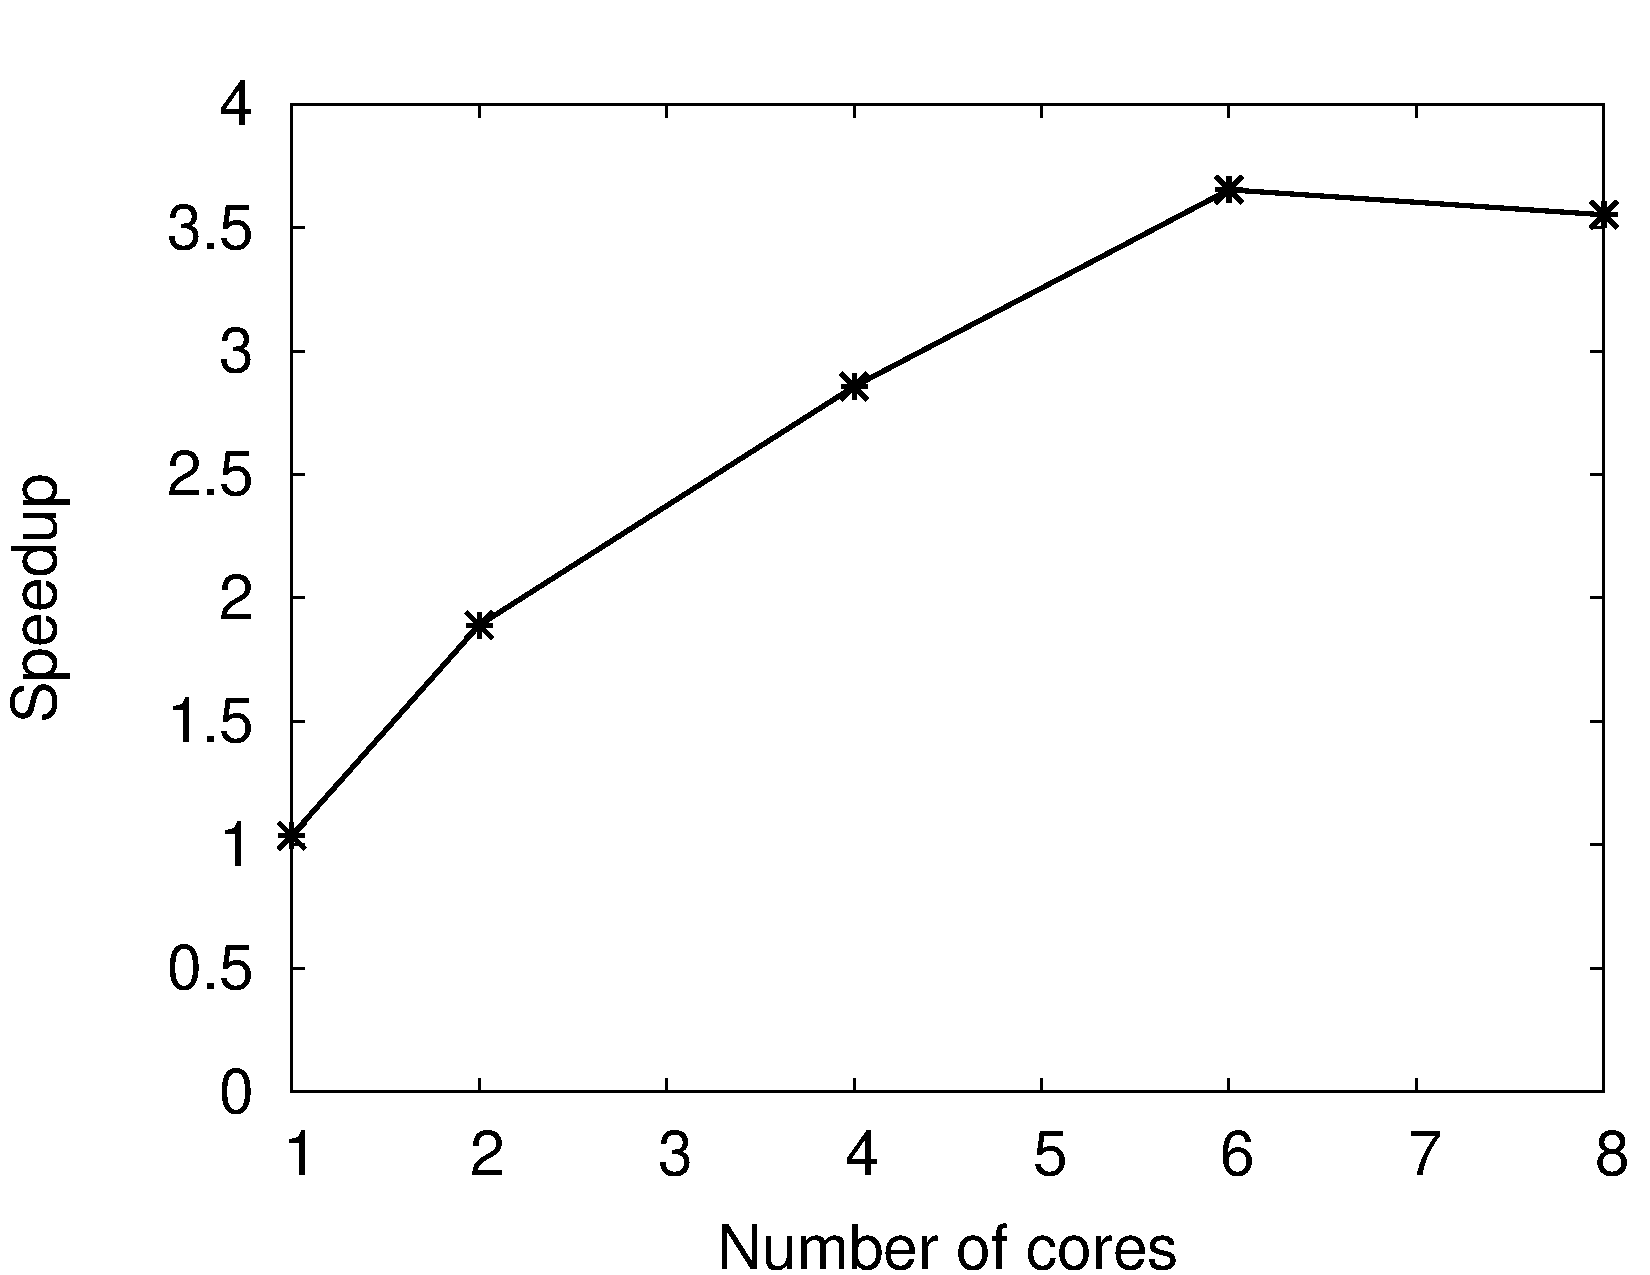
\includegraphics[width=5.8cm]{p4_scalability}
\caption{Speedup as a function of \#core}
\label{fig:scalability}
\end{figure}

{\bf Question P5.}
LBFGS (to be exact, the LMVM algorithm in TAO) keeps a number of previous gradients to approximate the inverse of the Hessian.
Call this number $p$ (default is 5 in TAO).
Although a larger value of $p$ leads to more accurate approximation, it also incurs higher computational cost.
So there seems to be a delicate tradeoff.
Set \#core to 4, and fix $\lambda$ to the optimal value in Question P2.
Vary the value of $p$ in $\{1, 5, 20\}$ ($p=5$ has already been done in previous questions).
To set $p$ to 1, just append the following to the command line in Question P1:

\verb!-tao_lmm_vectors 1!

Reproduce the plot in Question P2 for this optimal $\lambda$.
Still use ``\verb!-n 3 -loss CRF -tol 1e-3!".
But instead of plotting 3 figures (for the three values of $p$),
plot 3 curves in a single figure.
What conclusion can be drawn?

{\bf Solution P5.}

The results is shown in \ref{fig:LBFGS}, still with $\lambda$ = {\sf 1e-4}. From the plot we can see that when $p=1$, the object value drops slower than the other two curves, and it also takes longest time to converge. However, $p=5$ and $p=20$ does not have a big difference. Since larger $p$ may cause heavier computation cost, the default $p=5$ is a good balance between approximation accuracy and computation cost.

\begin{figure}[htbp!] 
\centering
\includegraphics[width=5.8cm]{p5_LBFGS}
\caption{Comparison of object value v.s. CPU time over $p \in \{${\sf 1, 5, 20}\}.}
\label{fig:LBFGS}
\end{figure}

{\bf Question P6.}
Do we really need to store the whole $\Ctr$ matrix in memory via storing $\cvec_{\text{local}}$ over all processes?
If yes, explain why.
If no, explain how this can be saved and how the computational performance will be impacted.

{\bf Solution P6.}

\textcolor{red}{Not done yet. May consider local and distributed difference.}

% =====================================================================================
\section{Torch: Tasks for Experiment}

{\bf Question T1.}
Run your implementation with the setting in the first 19 lines of \verb!train_CRF.lua!.
That is, use the first 100 words for training.
Copy and paste to your report
i) the first 11 lines (\ie\ 10 iterations) of the printout,
and
ii) the last line when it converges.
%
See \verb!sample_out_Torch.txt! for an example (only 4 lines are shown there, and the last line 49 is dummy).


For the questions below, you may create new files,
\eg\ if you feel it more convenient to collect SGD related code in a separate file.

{\bf Question T2.}
Implement the vanilla SGD algorithm and do not use \verb!optim.sgd!.
Also implement the Stochastic Average Gradient method with Non-Uniform Sampling (SAG-NUS) introduced by
\vspace{0.5em}

Non-Uniform Stochastic Average Gradient Method for Training Conditional Random Fields.
M. Schmidt, R. Babanezhad, M.O. Ahmed, A. Defazio, A. Clifton, A. Sarkar. AISTATS, 2015.
%
Their talk and Matlab code (for reference) can be found at
\verb!http://www.cs.ubc.ca/~schmidtm/Documents!.


Now for each $\lambda \in$ \verb!{1e-2, 1e-4, 1e-6}!,
plot a figure that that compares the three methods (LBFGS, SGD, SAG-NUS) over the training objective value.
See Figure \ref{fig:compare_sgd} for made-up plots.
Still use the first 19 lines of \verb!train_CRF.lua! for the problem setting.
However, {\bf you may now tune the parameters of the solvers.}
This includes, but not limited to, the \verb!optimState! structure in \verb!train_CRF.lua! for LBFGS,
as well as the step size rules for SGD and SAG-NUS.
Use whatever parameter that you feel is good for this problem,
and mention them in the report.
What conclusion can be drawn from these figures?

Note it can be expensive if we compute the objective value after \emph{each single} update of SGD/SAG-NUS.
So you may compute the value every 1000 updates (or pick a frequency that you feel reasonable).
The training set is again the first 100 words,
and SGD/SAG-NUS randomly picks one out of them at each step.


\begin{figure}[t]
\centering
\subfigure[$\lambda =$ {\sf 1e-2}]{
\includegraphics[width=5cm]{obj_Torch}}
~~
\subfigure[$\lambda =$ {\sf 1e-4}]{
\includegraphics[width=5cm]{obj_Torch}}
~~
\subfigure[$\lambda =$ {\sf 1e-6}]{
\includegraphics[width=5cm]{obj_Torch}}
\caption{Comparison of LBFGS, SGD, and SAG-NUS over $\lambda \in \{${\sf 1e-2, 1e-4, 1e-6}\}.}
\label{fig:compare_sgd}
\end{figure}


{\bf Question T3.}
What is your general experience of tuning the parameters of the solvers in {\bf Question T2}?
You do not need to be exhaustive, and just briefly describe what you tried and what you found.

{\bf Question T4.}
The advantage of stochastic optimization lies in the low cost per step.
Batch solvers like LBFGS require a lot of computation to process the whole data set,
which made it computationally challenging to train on the entire 3438 words.
So in the previous questions, we only used the first 100 words for training.
Now let us try SGD and SAG-NUS on the whole training set by randomly picking a word out of the {\bf 3438 words}.

Fix the value of $\lambda$ to what you used in {\bf Question P3},
whose results were given in Figures \ref{fig:letter_err} and \ref{fig:word_err}.
Re-produce Figure \ref{fig:word_err} (word-wise error) but do \emph{not} include the training error any more.
Instead, include the test error of LBFGS, SGD, and SAG-NUS.
Now it should look like Figure \ref{fig:compare_word_err}.

\begin{figure}[t]
\centering
\includegraphics[width=5cm]{error_Torch}
\caption{Comparison of word-wise error on the test data for $\lambda=$???.}
\label{fig:compare_word_err}
\end{figure}

The result of LBFGS is just copied from the PETSc results.
However, its timing was based on running on the cluster with multiple cores,
and is therefore not comparable with that of SGD/SAG-NUS which use Torch on a single core.
So we changed the x-axis in Figure \ref{fig:compare_word_err} to the \emph{effective number of passes}, which is essentially how many passes the solvers have swept over the entire training set.
For LBFGS, it is the 5-th number (integer) in the printout shown in {\bf Question P1}.
For SGD/SAG-NUS, it is the number of words sampled so far divided by 3438
(\#words in the training set).
Again for stochastic methods, the error can be computed every, say, 1000 steps.

What conclusions can be drawn from the plot?

{\bf Extra credit.}
You may also plot a similar figure for the test letter-wise error, and that will earn you extra 10 points out of 100.



\iffalse

memo

\begin{verbatim}
x = torch.ones(3,3)
y = x:sub(1,2)
y = torch.zeros(2,3)

th> y
 0  0  0
 0  0  0
[torch.DoubleTensor of size 2x3]

th> x
 1  1  1
 1  1  1
 1  1  1
[torch.DoubleTensor of size 3x3]
\end{verbatim}

read the first 53 lines of \verb!torch/pkg/optim/lbfgs.lua! to understand the parameters for lbfgs.


The return values of require, e.g. \verb!require "nn"!, are cached so a file is run at most once,
even when require'd many times.
So if you edit the module and rerun the code that uses this module via "require",
your changes won't be picked up.
You may quit torch and restart it to re-load the module.
You may ``unrequire" by \url{http://lua-users.org/lists/lua-l/2009-03/msg00587.html}

\newpage
\fi


\end{document}
